\section{Real Data}

\begin{frame}[fragile] % Need to use the fragile option when verbatim is used in the slide
    \frametitle{Real Data}
    \textbf{Data}: Titanic data
    \newline \textbf{Method used}: 
    \begin{enumerate}
        \item Random Forest
        \item AdaBoost
        \item Gradient Boosting Classifier
    \end{enumerate}
    \newline \textbf{Goal}: Given features of passengers predict which passengers survived the Titanic shipwreck 
    

\end{frame}
    
%------------------------------------------------

\begin{frame}[fragile] % Need to use the fragile option when verbatim is used in the slide
    \frametitle{Real Data: results}
 
\begin{columns}[c] % The "c" option specifies centered vertical alignment while the "t" option is used for top vertical alignment
    
    \column{.33\textwidth} % Left column and width
    Random Forest
    \newline Accuracy: ~84,32\%
    \begin{center}		
		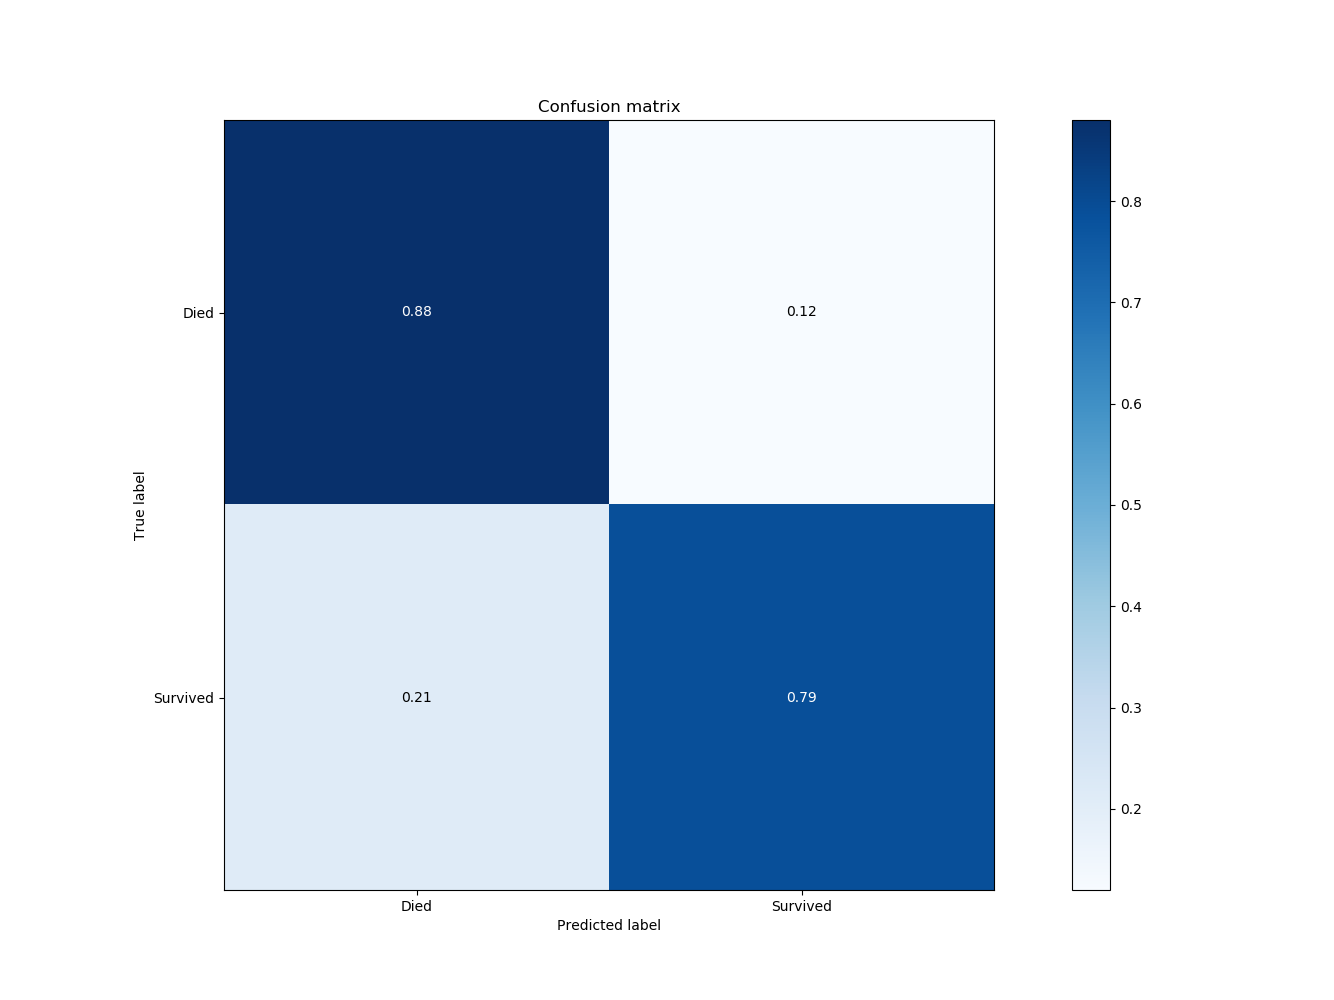
\includegraphics[height=0.3\textheight]{images/confusion_matrix_random_forest.png}
	\end{center}
    
    \column{.33\textwidth} % Central column and width
    AdaBoost
    \newline Accuracy: ~82.8\%
	\begin{center}		
		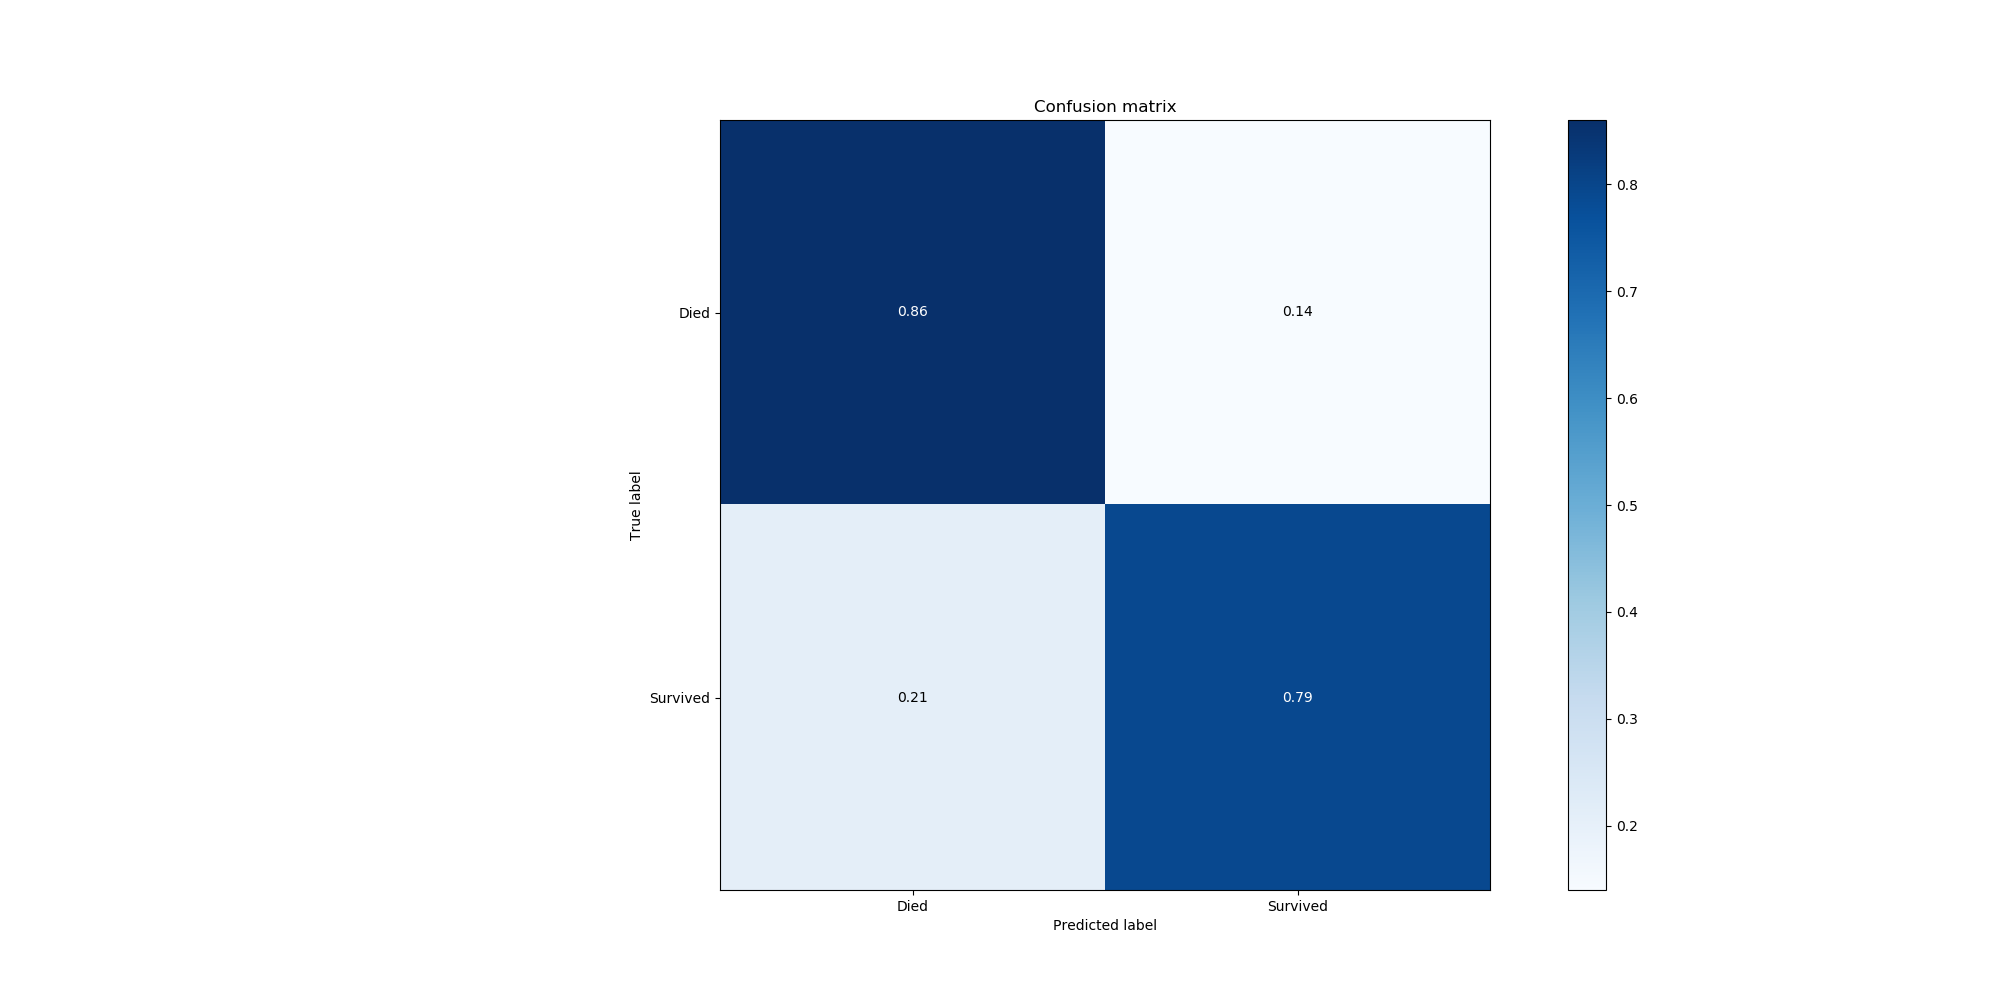
\includegraphics[height=0.3\textheight]{images/confusion_matrix_adaboost.png}
	\end{center}
	
    \column{.33\textwidth} % Right column and width
    Gradient Boosting
    \newline Accuracy: ~82,8\%
	\begin{center}		
		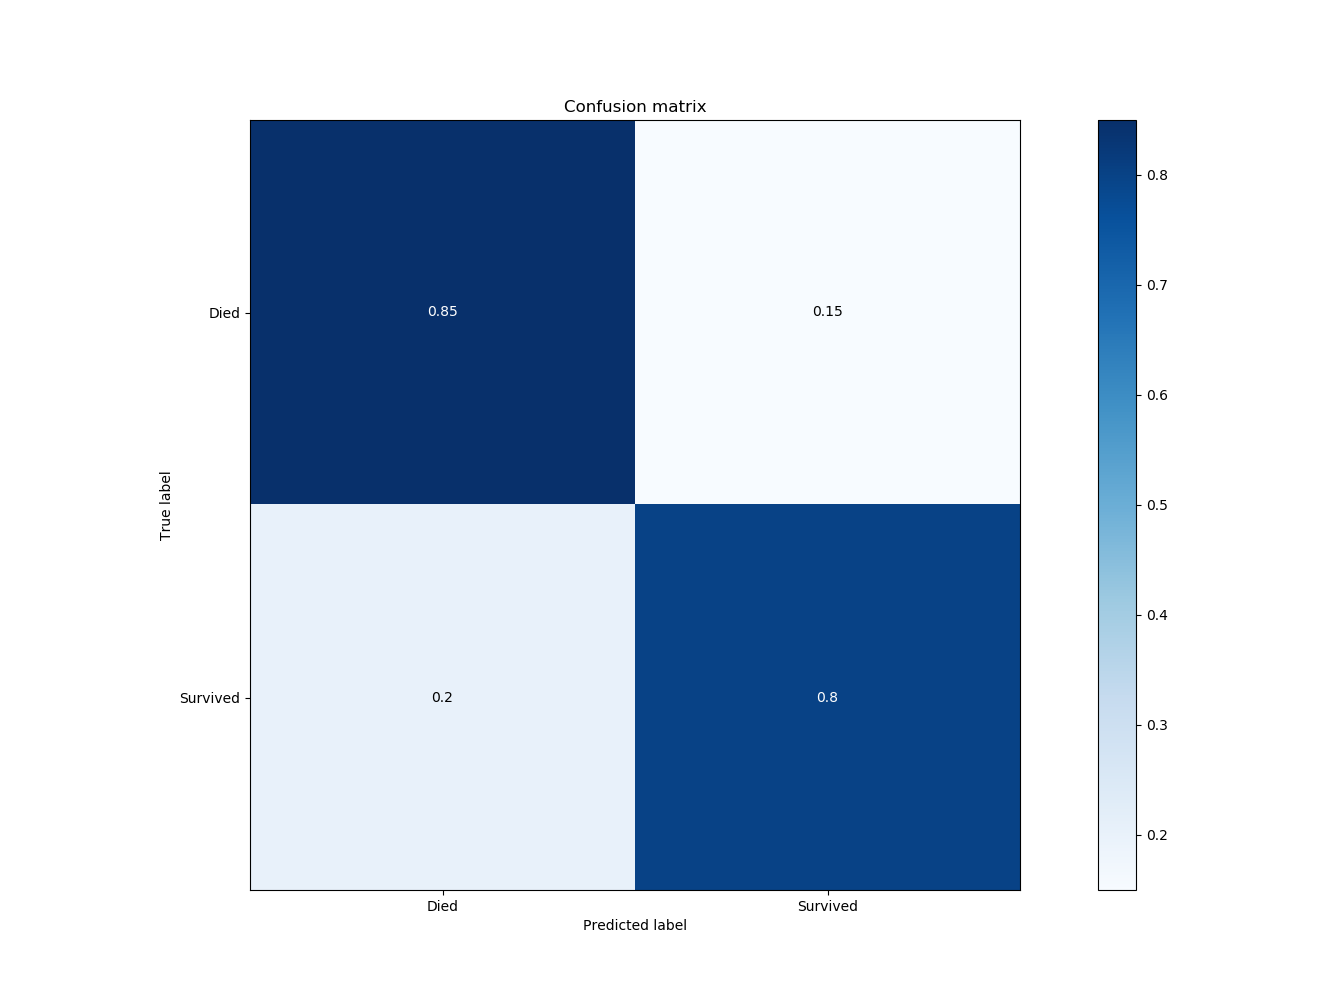
\includegraphics[height=0.3\textheight]{images/confusion_matrix_gradient_boosting.png}
	\end{center}

    
    \end{columns}


\end{frame}